% !TEX root = ../entropy.tex

\section{Interpreting entropy}%
\label{sec:interpreting_entropy}

To see how we can interpret entropy as the predictability of a user's spending behaviour, it is useful to have a more complete
understanding of Equation~\ref{equ:entropy}. The building blocks of entropy is
the information content of a single event. The key intuition
\citet{shannon1948mathematical} aimed to capture was that learning of the
occurrence of a low-probability event is more informative than learning of the
occurrence of a high-probability event. The information of an event $I(E)$ is
thus inversely proportional to is probability $p(E)$. One way to capture this
would be to define the information of event E as $I(E) = \frac{1}{p(E)}$. Yet
this implied that an event that is certain to occur had information 1, when it
would make sense to have information 0. To remedy this (and also satisfy
additional desireable characteristics of an information function), Shannon
proposed using the log of the expression. Hence, the information of event E,
often called \textit{Shannon information}, \textit{self-information}, or just
\textit{information}, is defined as:

\begin{equation}
    I(E) = log\left(\frac{1}{p(E)}\right) = -log(p(E)).
\end{equation}

The choice of the base for the logarithm varies by application and determines
the units: base 2 means that information is expressed in bits; the natural
logarithm, another popular choice, expresses information in \textit{nats}.

Entropy, often called \textit{Information entropy}, \textit{Shannon entropy},
or just \textit{entropy}, is the information of a random variable, $X$, and
captures the expected amount of information of an event drawn at random from
the probability distribution of the random variable. It is calcualted as:

\begin{equation}
    H(X) = -\sum_x p(x) \times log(p(x)) = \sum_x p(x)I(x) = \mathbb{E} I(x).
\end{equation}

For a single event, the key intution was that the less likely an event, the
more information is conveyed when it occurs. The related idea for distributions
is similar: the less skewed a distribution of a random variable, the less
certain the realised value of a single draw from the distribution, the higher
is entropy - the maximum entropy distribution is the uniform distribution.


\section{Entropy components}%
\label{sec:entropy_components}

Figure~\ref{fig:entropy_components} shows the empirical relationship with our
48-categories-based unsmoothed entropy variable and these three
components.\footnote{To highlight the main features of the relationships we
have trimmed the component values at the 95th percentile.} We can see that for
the values we observe in the dataset, entropy increases monotonically in the
number of unique spending categories with positive frequency counts, has no
clear relationship with the standard deviation of those counts, and increases
in the number of total spending transactions up to about 175 transaction,
before being increasingly determined by other elements thereafter.

\begin{figure}[ht]
    \centering 
    \caption{Correlation of entropy with its components}
    \label{fig:entropy_components}
    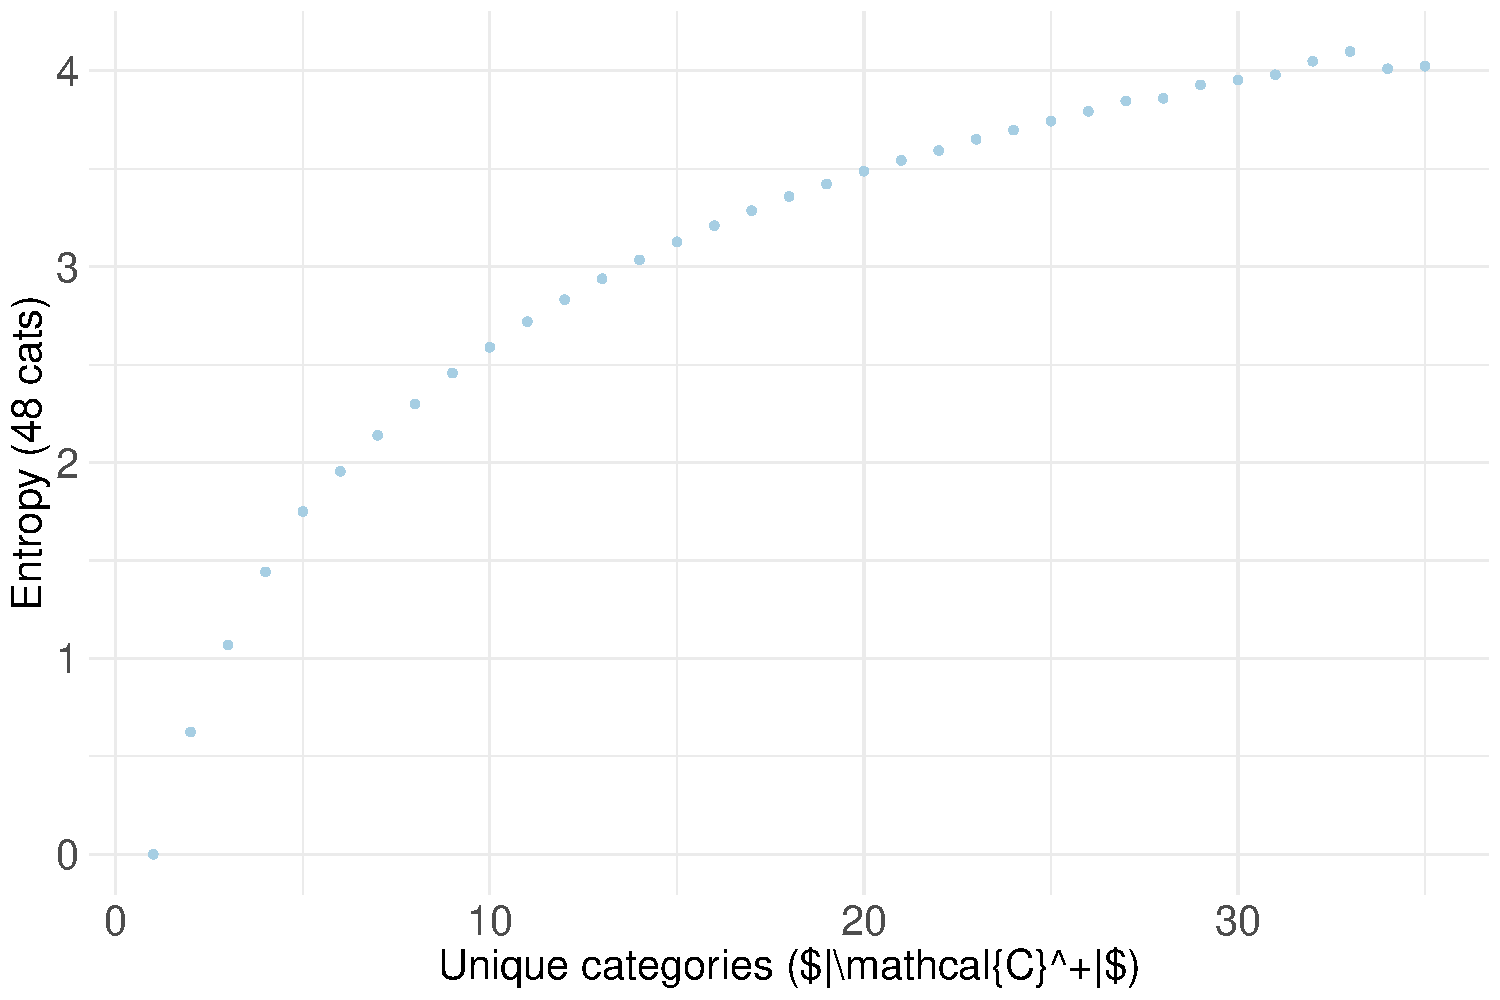
\includegraphics[width=.32\textwidth]{\figdir/scatter_entropy_nunique_tag_spend.pdf}
    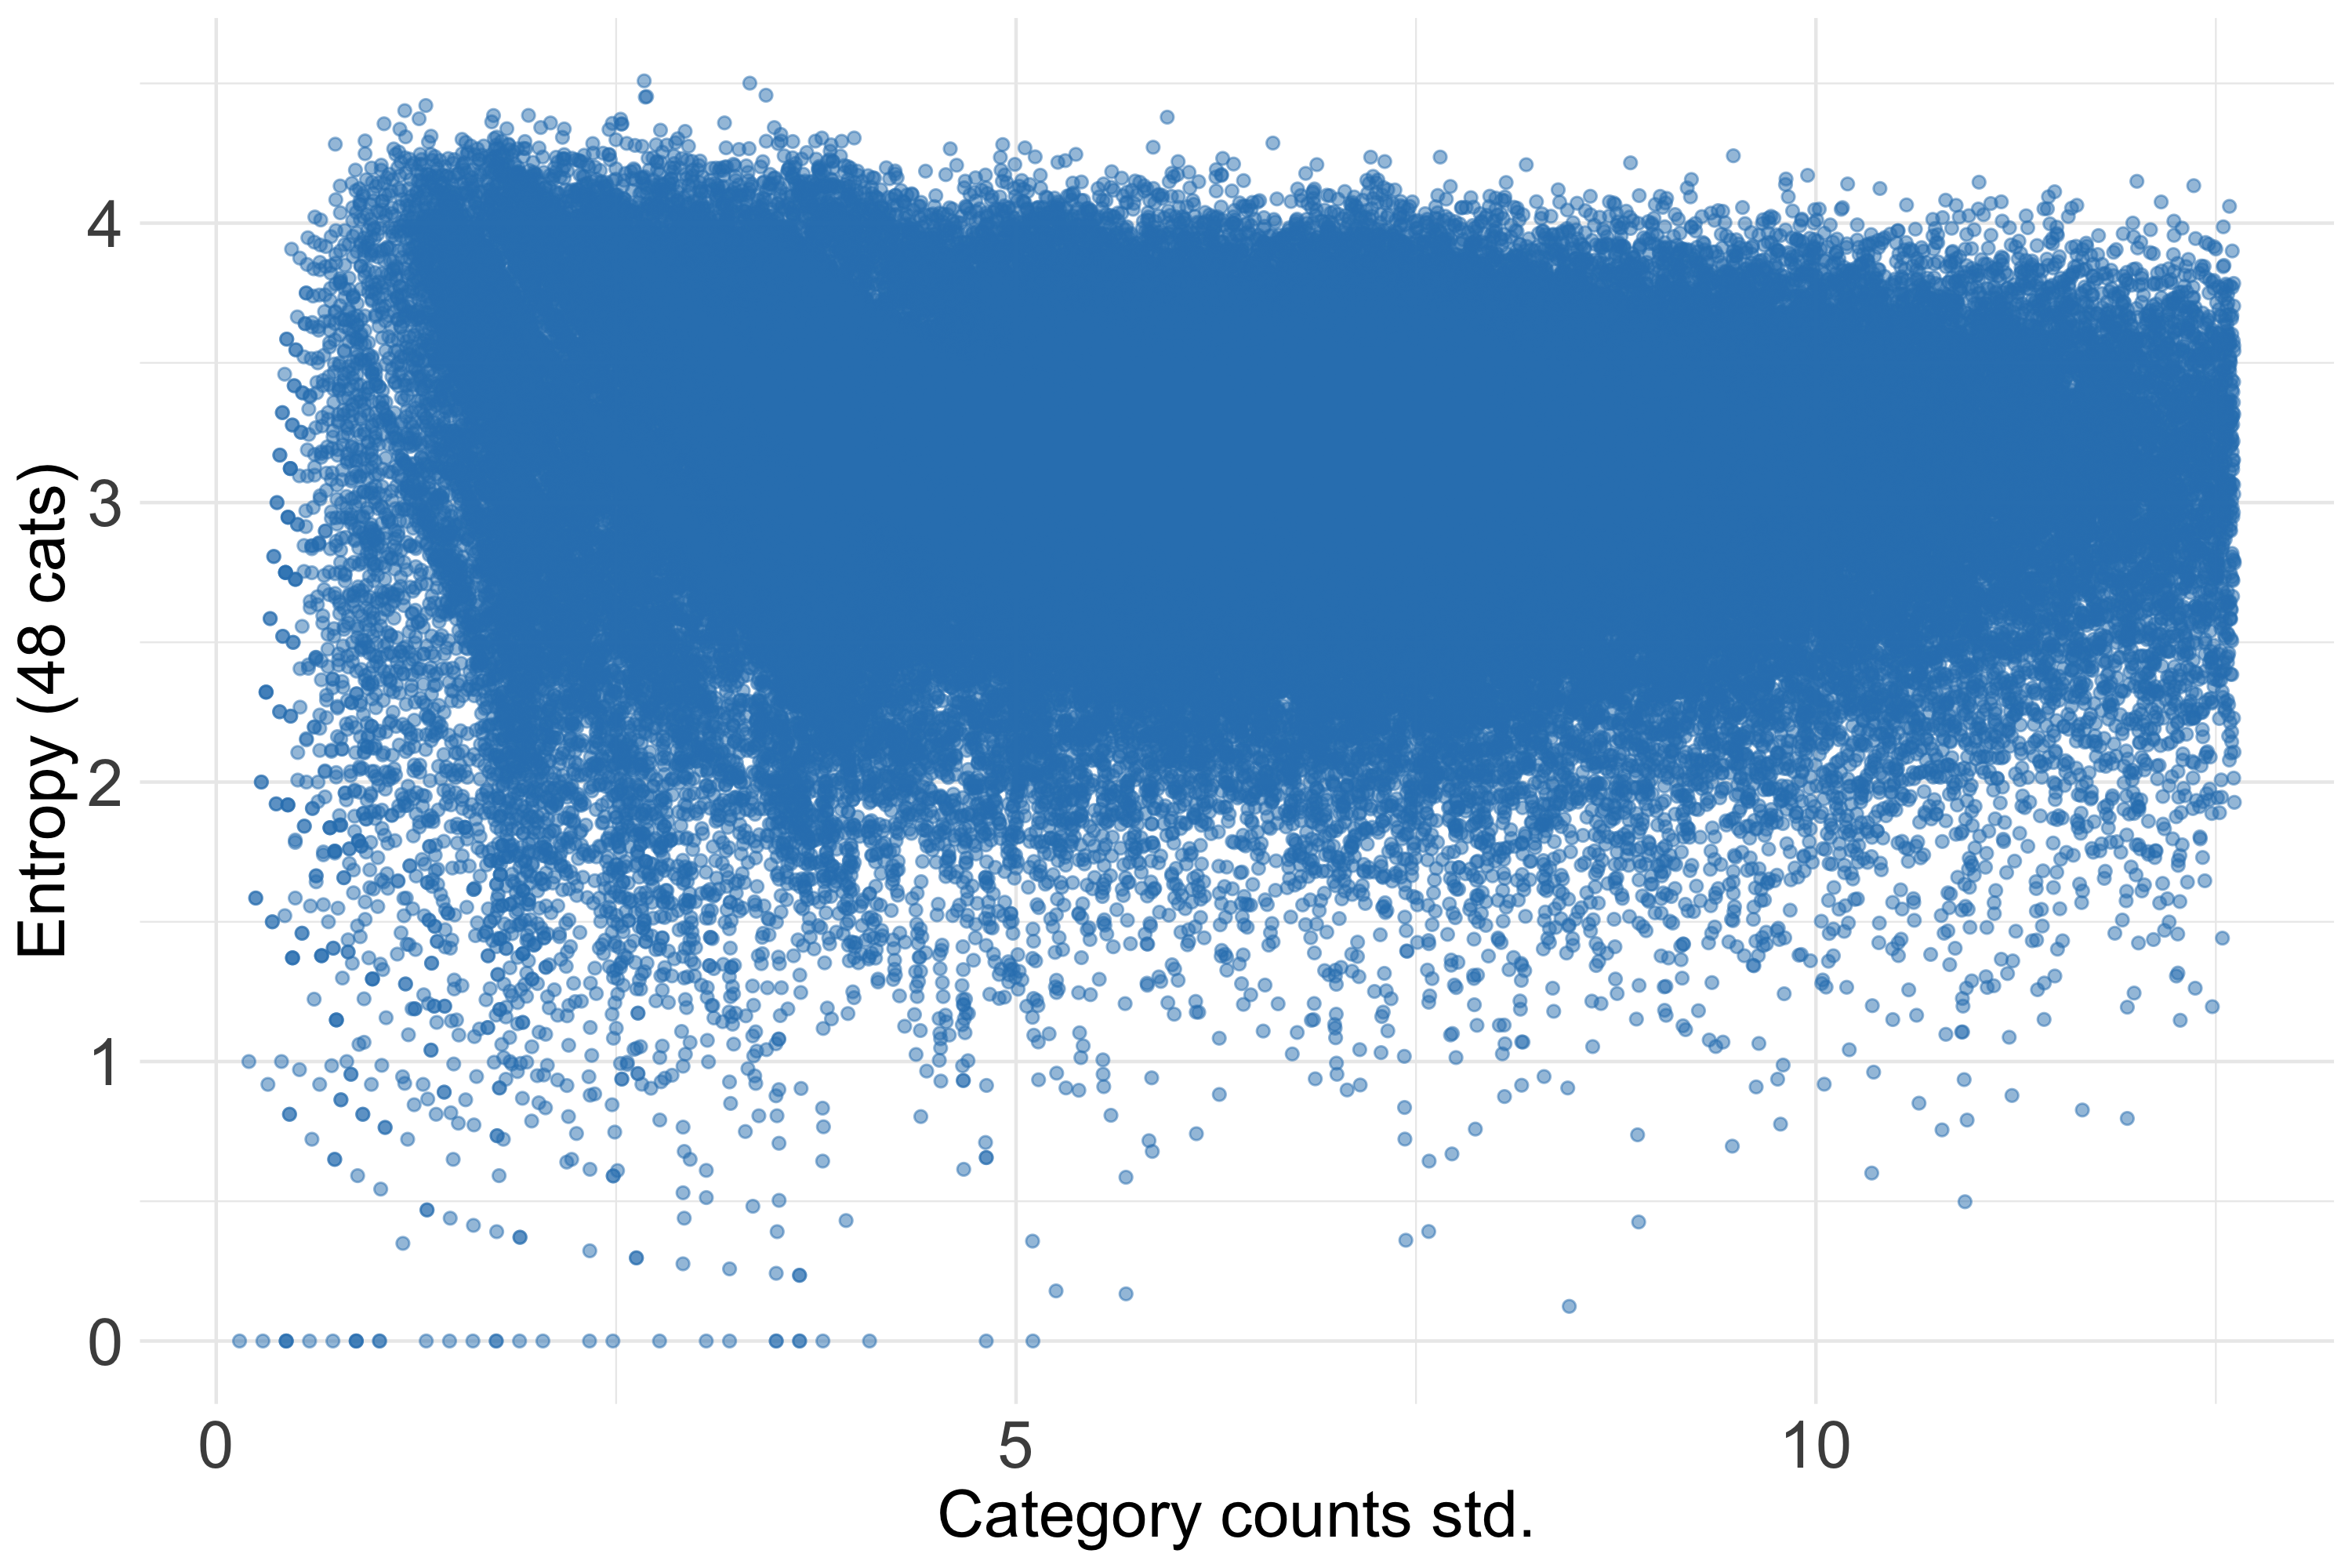
\includegraphics[width=.32\textwidth]{\figdir/scatter_entropy_std_tag_spend.pdf}
    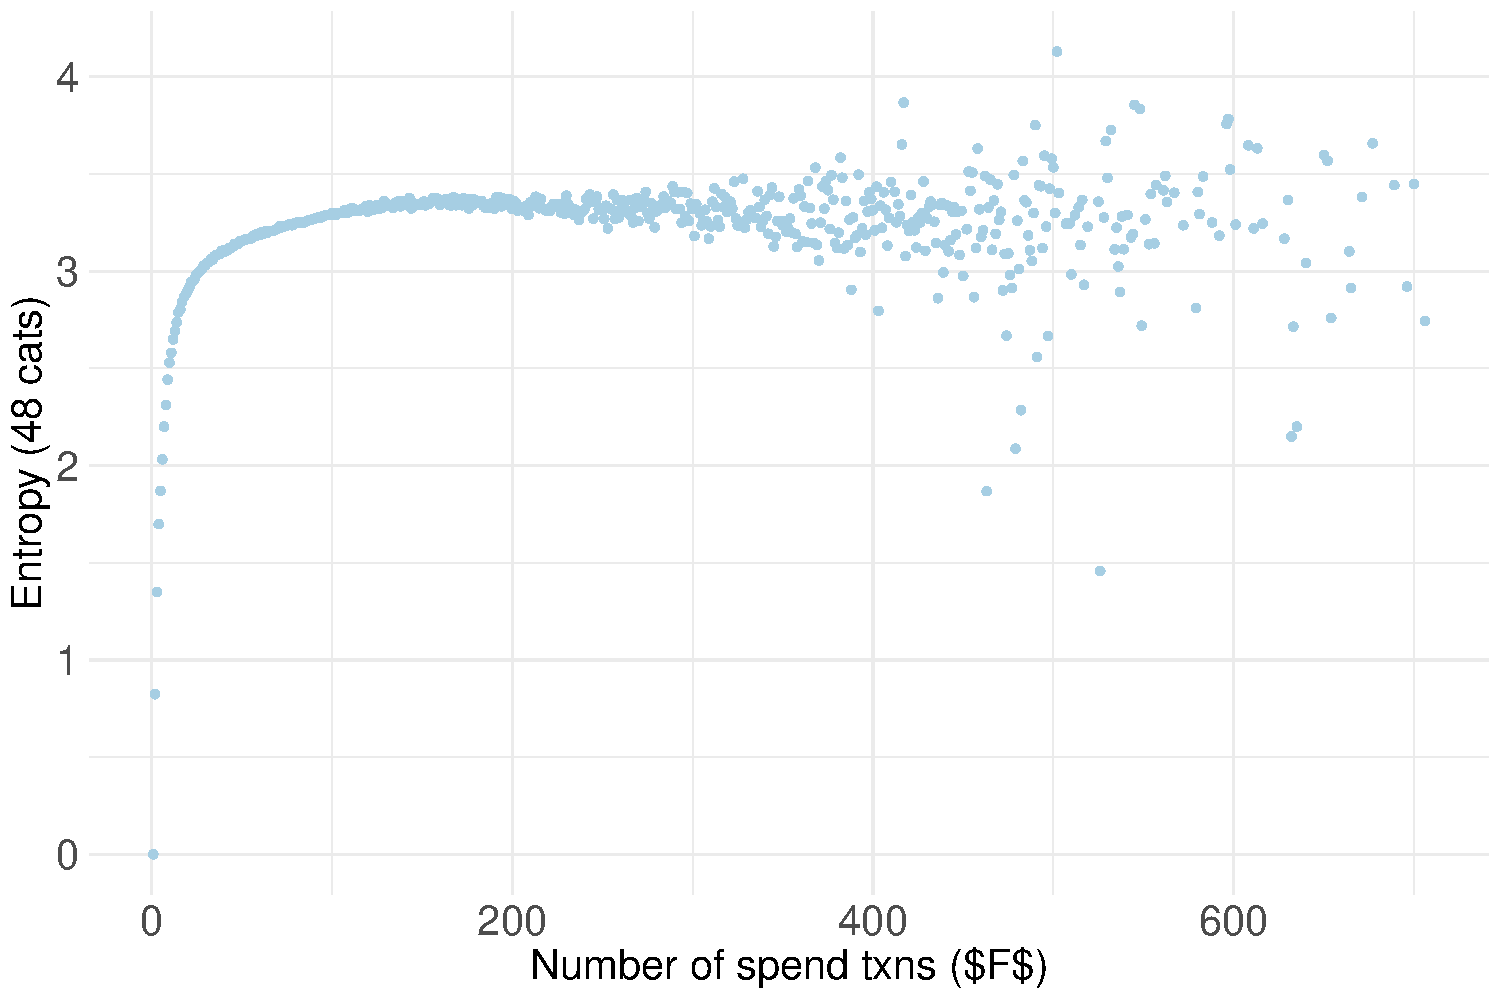
\includegraphics[width=.32\textwidth]{\figdir/scatter_entropy_txns_count_spend.pdf}
    \fignote{\textwidth}{Correlation of 48-categories-based unsmoothed entropy
    with its three main components: the number of unique spending categories
with positive frequency counts (left), the standard deviation of those
frequency counts (middle), and the number of total spend transactions (left).}
\end{figure}


\section{Effect of smoothing on entropy}%
\label{sec:effect_of_smothing_on_entropy}

\begin{figure}[ht]
    \centering 
    \caption{Effect of smoothing on entropy}
    \label{fig:scatter_facets_txns_count_spend_q}
    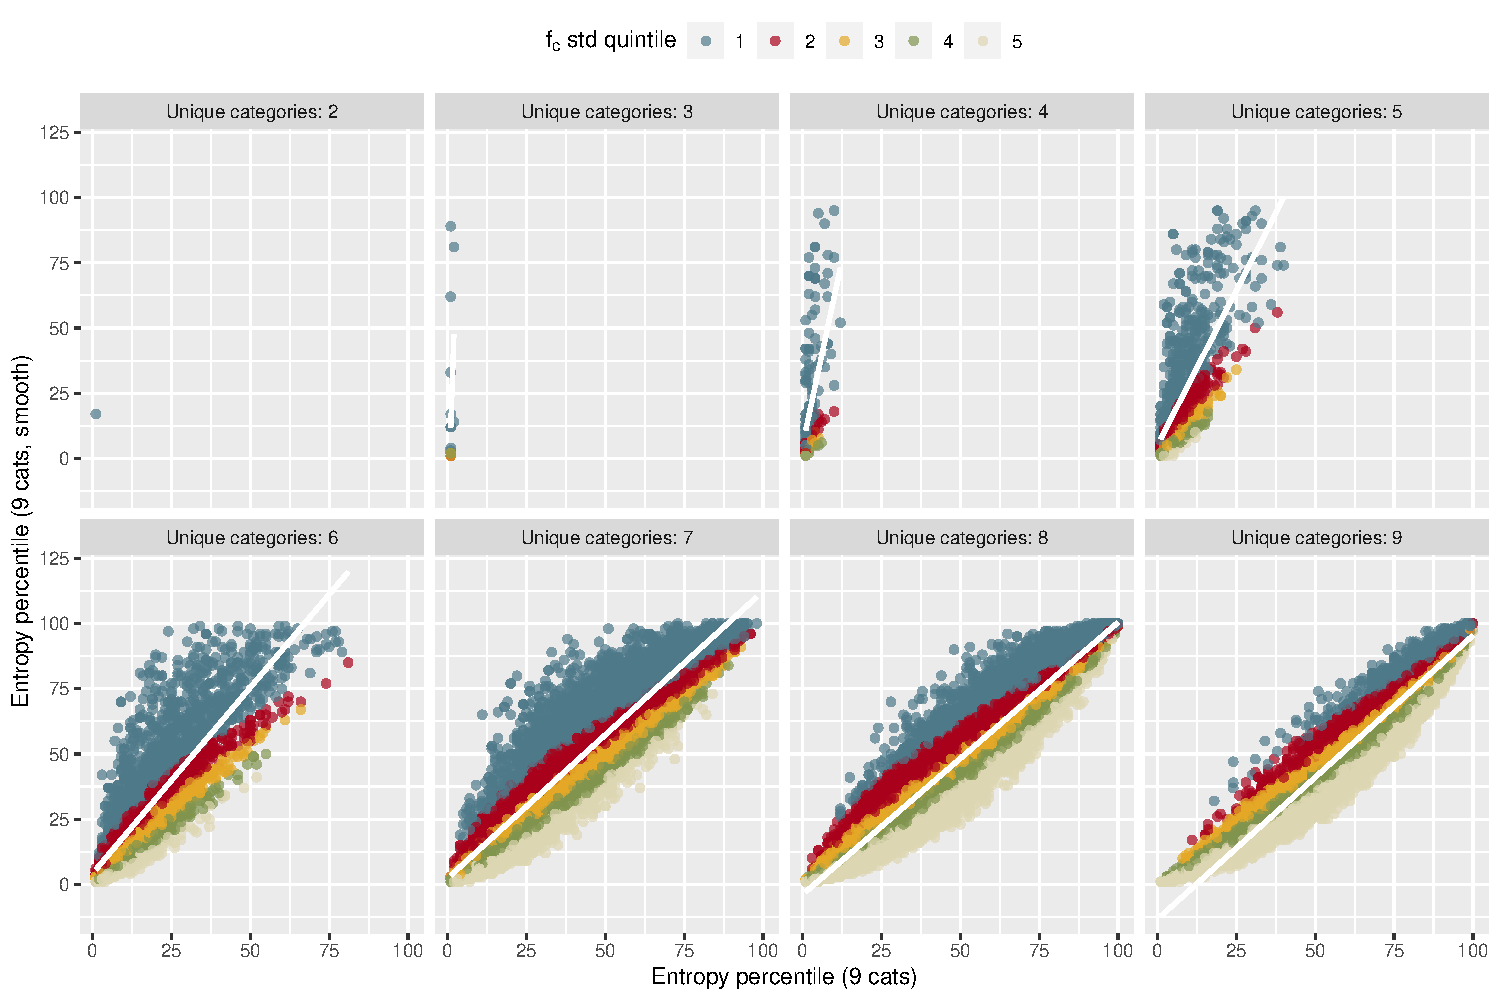
\includegraphics[width=\textwidth]{\figdir/scatter_facet_std_tag_q.pdf}
    \fignote{\textwidth}{Percentile ranks of 9-category-based unsmoothed and
    smoothed entropy separated by the number of categories with positive
frequency counts. White reference lines indicate equal percentile ranks.
Colours indicate the quintile of the total number of spending transactions.}
\end{figure}

